\documentclass[../r.tex]{subfiles}

\begin{document}

\section{Teaching Assistant Experience}
Created assignments, lead discussion groups, graded (exams, quizzes, projects), and held office hours for the following: Analysis of Algorithms, 2x Penetration Testing, Distributed Operating Systems, 2x Programming Fundamentals 2, Applications of Discrete Structures, Introduction to Digital Arts and Sciences, 2x Senior Project, Software Engineering.  Here are some example assignments that I've created for students: \href{./TAing/fractals.pdf}{fractals}, \href{./TAing/Project3-Breakout.pdf}{breakout (game)}, \href{./TAing/rocket_lab.pdf}{rocket lab}.  And here are some animations: \href{https://twitter.com/randompast/status/1031298467744886785}{circle packing}, \href{https://twitter.com/randompast/status/1031242914112970753}{circle rendering}.  And, here's a neat tree approach to creating the Sierpinski Gasket and result from the circle packing demo.

\noindent
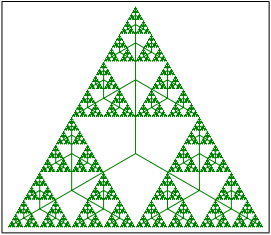
\includegraphics[scale=0.69]{../TAing/sierpiskigasket.png} 

\includegraphics[scale=0.3]{../TAing/einstein.jpeg} 

\end{document}